\chapter{The DSDM Lightweight Arm }
\label{sec:ExperimentalValidation}

\vspace{-5pt}
{ \Large Mechanical Design, Control and Software Architecture }

{
\begin{flushright}
\textit{"What I cannot create, I do not understand."} \\ 
\emph{-- Richard Phillips Feynman}
\end{flushright}
}
\vspace{10pt}

%\begin{flushright}
%\small"The test of all knowledge is experiment. Experiment is the sole judge of scientific truth." \\ \emph{Richard Phillips Feynman}
%\end{flushright}


This chapter present a novel 3-DoF robotic arm prototype using DSDM actuators, see Fig. \ref{fig:dsdm_arm_zoom} and Fig. \ref{fig:dsdm_arm}. The mechanical design of the DSDM actuators and the robotic arm is discussed, as well as the control and software implementation.

\begin{figure}[htb]
	\centering
		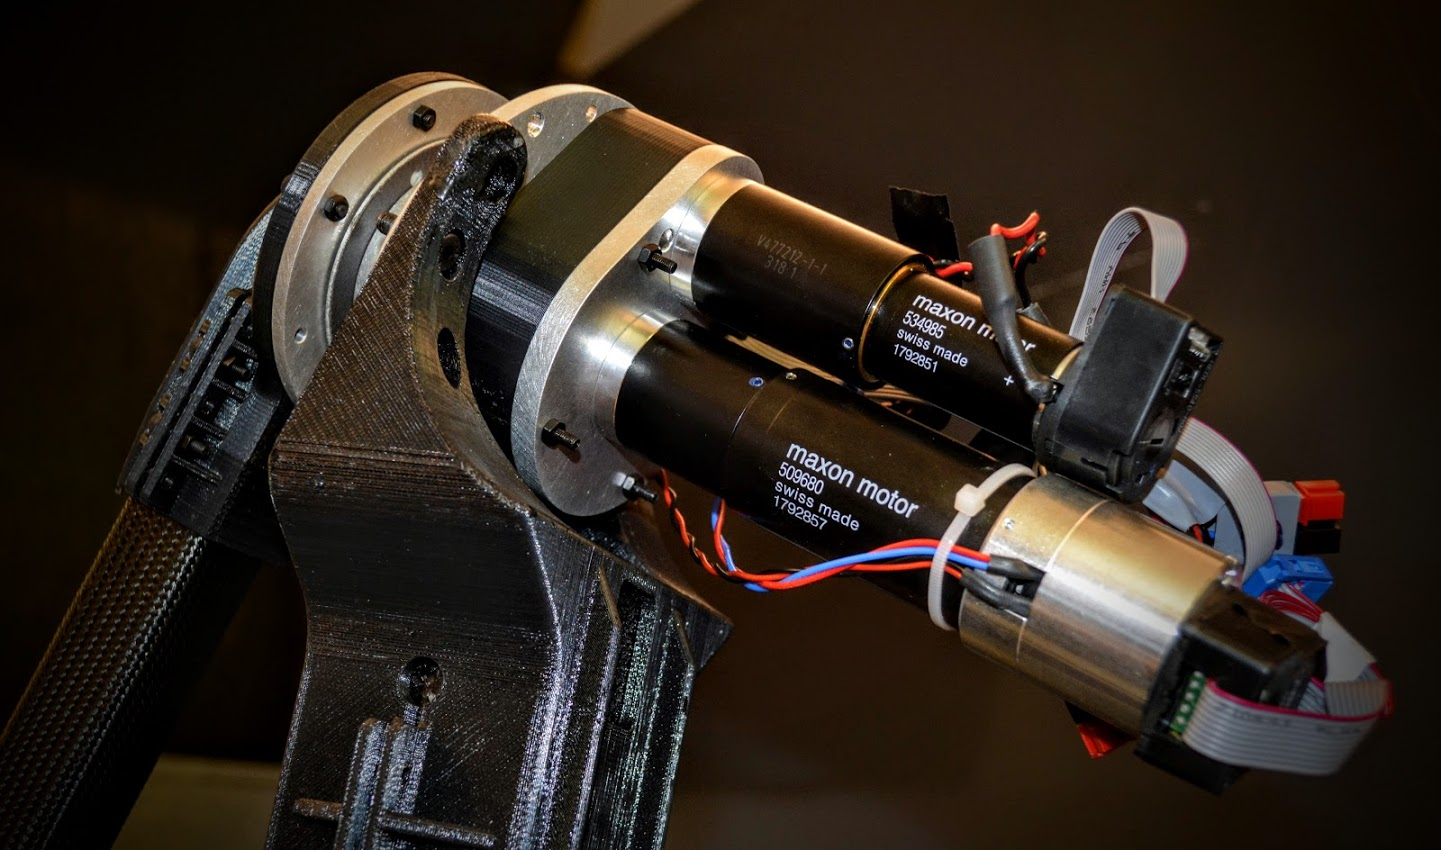
\includegraphics[width=0.70\textwidth]{arm_proto_zoom.jpg}
	\caption{Second joint of the DSDM-Arm}
	\label{fig:dsdm_arm_zoom}
\end{figure}

\begin{figure}[htp]
	\centering
		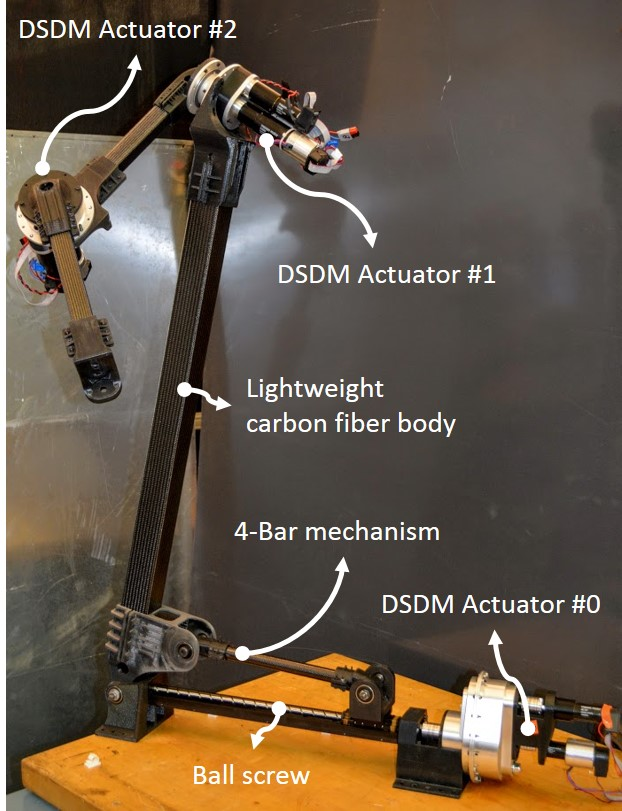
\includegraphics[width=0.95\textwidth]{arm_proto_3.jpg}
	\caption{DSDM-Arm: 3-DoF custom arm using 3 DSDM actuators}
	\label{fig:dsdm_arm}
\end{figure}

\section{Mechanical Design}

This section describes the mechanical design of the arm. The goal was to develop a research platform to validate experimentally the ideas proposed in this thesis, but also to demonstrate the advantages of robotic systems with variable gear-ratio actuators. This arm is thus design to be light-weight compared to robotic arm of similar size, maximum speeds and forces. 

\subsection{DSDM Actuator Design}
\label{sec:ActuatorDesign}
 
Three actuator prototypes were developed for the shoulder, elbow and wrist DoF of the arm, with different mechanical advantages. The shoulder actuator is designed to drive a ballscrew, for a large efficient reduction, and the others actuators are embedded into revolute joints. 

\subsubsection{3-port differential gear-box}

One of the main design challenge arising from the DSDM architecture, is the mechanical implementation of the differential junction between the two motors and the output. In a car powertrain the differential (required to allow a single motor to transmit torque to two wheels rotating at different velocities) is typically implemented with bevel gears. The approach taken here is different, a planetary set of gear is used, where the ring-gear (typically fixed) is mounted on bearing and connected to a parallel shaft. The connection to the parallel shaft is done with a stage of spur gears, with external gear teeth on the ring-gear assembly and another spur gear on the parallel shaft, see Fig. \ref{fig:diff1}. This configuration allows for all the shafts in the transmission and the motors to be parallel, which simplify the design. In all prototypes, the correspondence between planetary ports and inputs/outputs is the same, and described by Table \ref{tab:PlanetaryGearingInputsAndOutput}. This correspondence is picked to match the kinematic relationships arising from sizing constraints in the gearing. From eq. \eqref{eq:kinematic}, with a typical ratio in the planetary of $N=3$ (planet-gear size over internal ring-gear size), and a reduction ratio of $r_2=4$ for the parallel shaft connection (smaller $r_2$ would require a large distance between parallel shafts leading to larger transmission volume and larger $r_2$ is difficult to achieve in a single spur-gear stage), it leads to:
%
\begin{align}
	N \approx 3 \quad r_2 \approx 4 \quad\Rightarrow\quad R_1 = N+1 \approx 4 \quad R_2 = r_2 \frac{N+1}{N} \approx 5
\end{align}
%
Hence, the largest reduction through the differential gearing is assigned to M2 and the smallest reduction to M1. This choice is also motivated by the fact that the path going through the ring-gear and the additional stage, would lead to more friction and inertia which is less a concern for high-force mode than for high-speed mode. 

\begin{table}[htbp]
	\centering
		\begin{tabular}{ c c }
			\hline
			Rotating assembly & Role \\
			\hline \hline
			Planet carrier assembly & Actuator output \\
			Parallel shaft (connected to the ring-gear) & Motor M2 input (high-force) \\
			Sun gear shaft          & Motor M1 input (high-speed) \\
			\hline
		\end{tabular}
	\caption{Planetary gearing inputs and outputs}
	\label{tab:PlanetaryGearingInputsAndOutput}
\end{table}

\begin{figure}[htp]
        \centering
				\subfloat[Linear Actuator]{ % intrinsic dynamics
				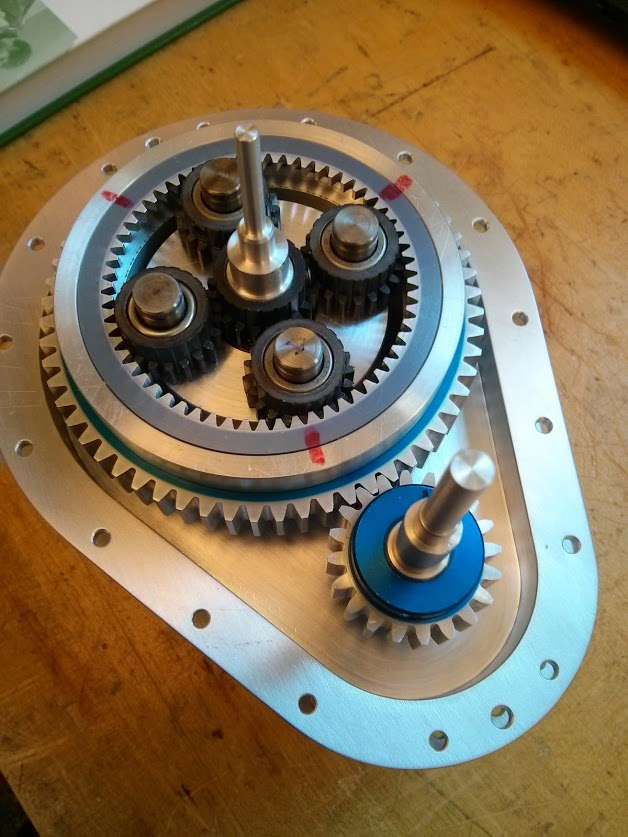
\includegraphics[width=0.40\textwidth]{gears.jpg} 
				\label{fig:diff1}}
				\hspace{+5pt}
        \subfloat[Revolute Joint]{ % intrinsic dynamics
				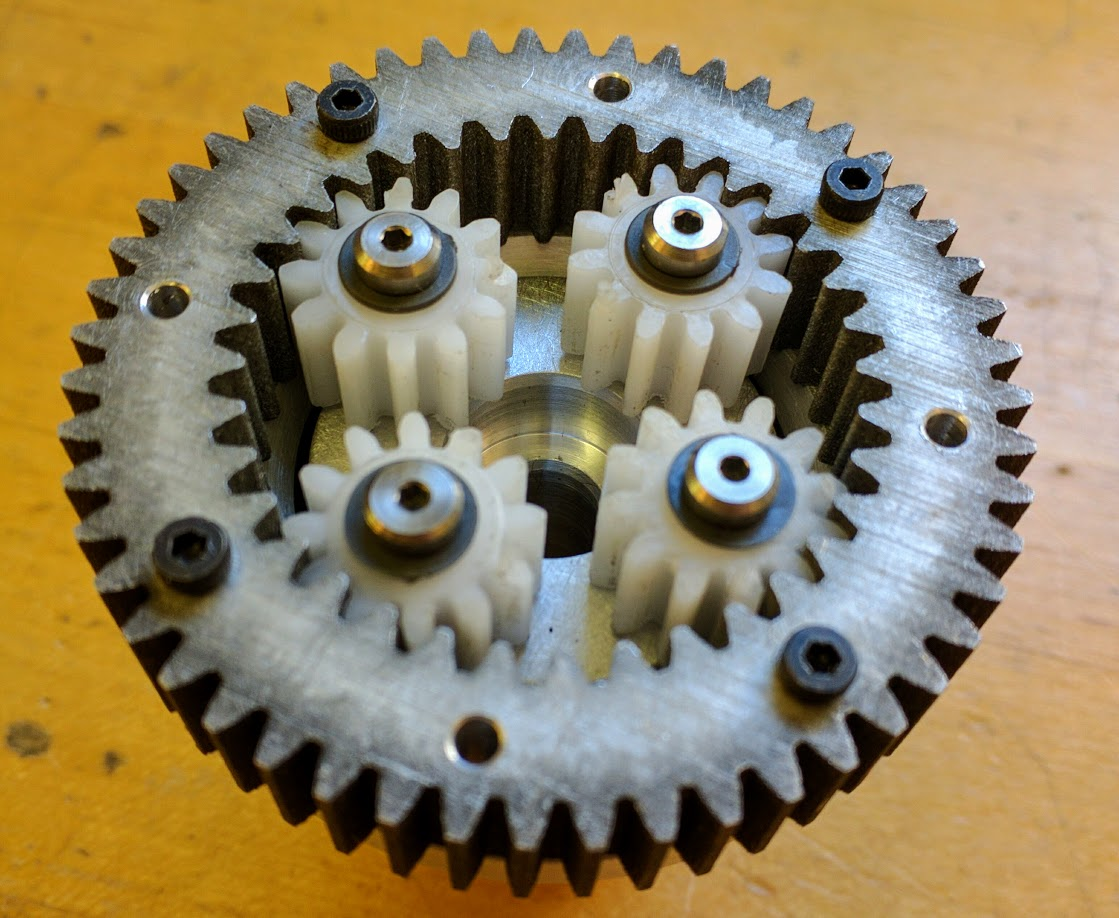
\includegraphics[width=0.50\textwidth]{gears_new.jpg}
				\label{fig:diff2}}
        \caption{Differential gear-box implemented with a planetary}
				\label{fig:differnentials}
\end{figure}

Fig. \ref{fig:diff1} shows the designed differential gearing for the linear actuator prototype and Fig. \ref{fig:diff2} shows the designed differential gearing for the revolute actuators. The first design (a) was using only off-the-shelf gears, which led to a big assembly. For the second design (b) a lot of effort was put into downsizing the assembly. For instance, custom ring gears with both internal and external gear teeth were designed, to minimize the diameter of the ring-gear assembly.

\subsubsection{Brake}

The second challenging mechanical component in a DSDM, is the brake. As discussed in Chapter, \ref{sec:MultipleSpeedActuationTechnology} control schemes can be used to bring M1 velocity to zero before engaging the brake, hence the brake only has to be a locking mechanism and does not have to be able to dissipate power. However, during high-force mode, large holding torques must be sustained. From eq. \eqref{eq:torque}, the holding torque requirement can be computed in term of desired maximum output force during high-force mode, or by the maximum M2 motor torque: 
%
\begin{align}
	\tau_{brake} = \frac{ \operatornamewithlimits{max} \left[ \tau_{output} \right] }{R_1} = \frac{ R_2 }{ R_1 } \operatornamewithlimits{max} \left[  \tau_2 \right]
	\label{eq:brakelim}
\end{align}
%
Hence, the design of the brake is coupled with the desired ratio between $R_1$ and $R_2$. If the high-force mode gear-ratio $R_2$ is 10 times greater than the high-speed mode gear-ratio $R_1$, than the brake must be able to hold torques 10 times greater than M2 maximum output torque. 

Because it allows for simpler and modular designs, it was decided to use off-the-shelf \textit{Maxon} motor brakes that can be mounted directly on a motor assembly. All actuator designs use the \textit{Maxon} motor brake AB-28, which have a holding torque capability of 0.4 Nm and weight 51 g. 


\subsubsection{Revolute Joint Actuators}

Fig. \ref{fig:dsdm_act} shows the prototype for a revolute DSDM actuator. The elbow and wrist actuator have the same design with the exception of using different gear-head for the motors, leading to overall different gear-ratios $R_1$ and $R_2$.
%
\begin{figure}[htp]
	\centering
		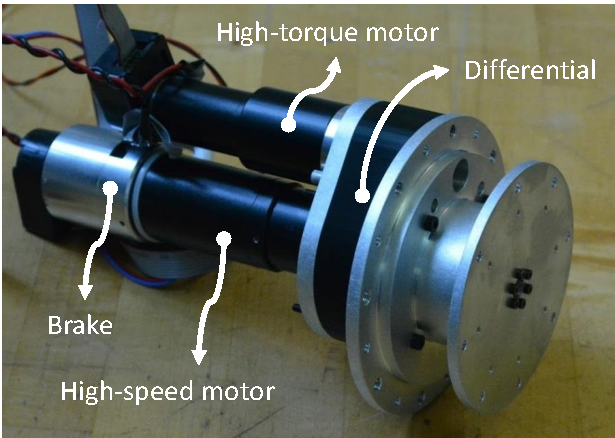
\includegraphics[width=0.70\textwidth]{dsdm_proto2.pdf}
	\caption{Revolute joint DSDM actuator prototype } %Max continuous torque of 40 Nm and maximum velocity of 100 RPM
	\label{fig:dsdm_act}
\end{figure}
%
The design for the revolute actuator consists of a custom housing holding both the planetary differential and support bearings for the output. Discrete \textit{Maxon} motors with gear-heads of the series GP32 can be attached to the back of the gear-box. It is thus possible to attach a wide-range of motor, from 20 watts to 200 watts, and with a wide range of additional gear-head reduction. Fig. \ref{fig:dsdm_section} shows the internal architecture of the system with a section view of the CAD model, and Fig. \ref{fig:dsdm_parts} shows all the internal parts of the actuator assembly. 

\begin{figure}[htp]
	\centering
		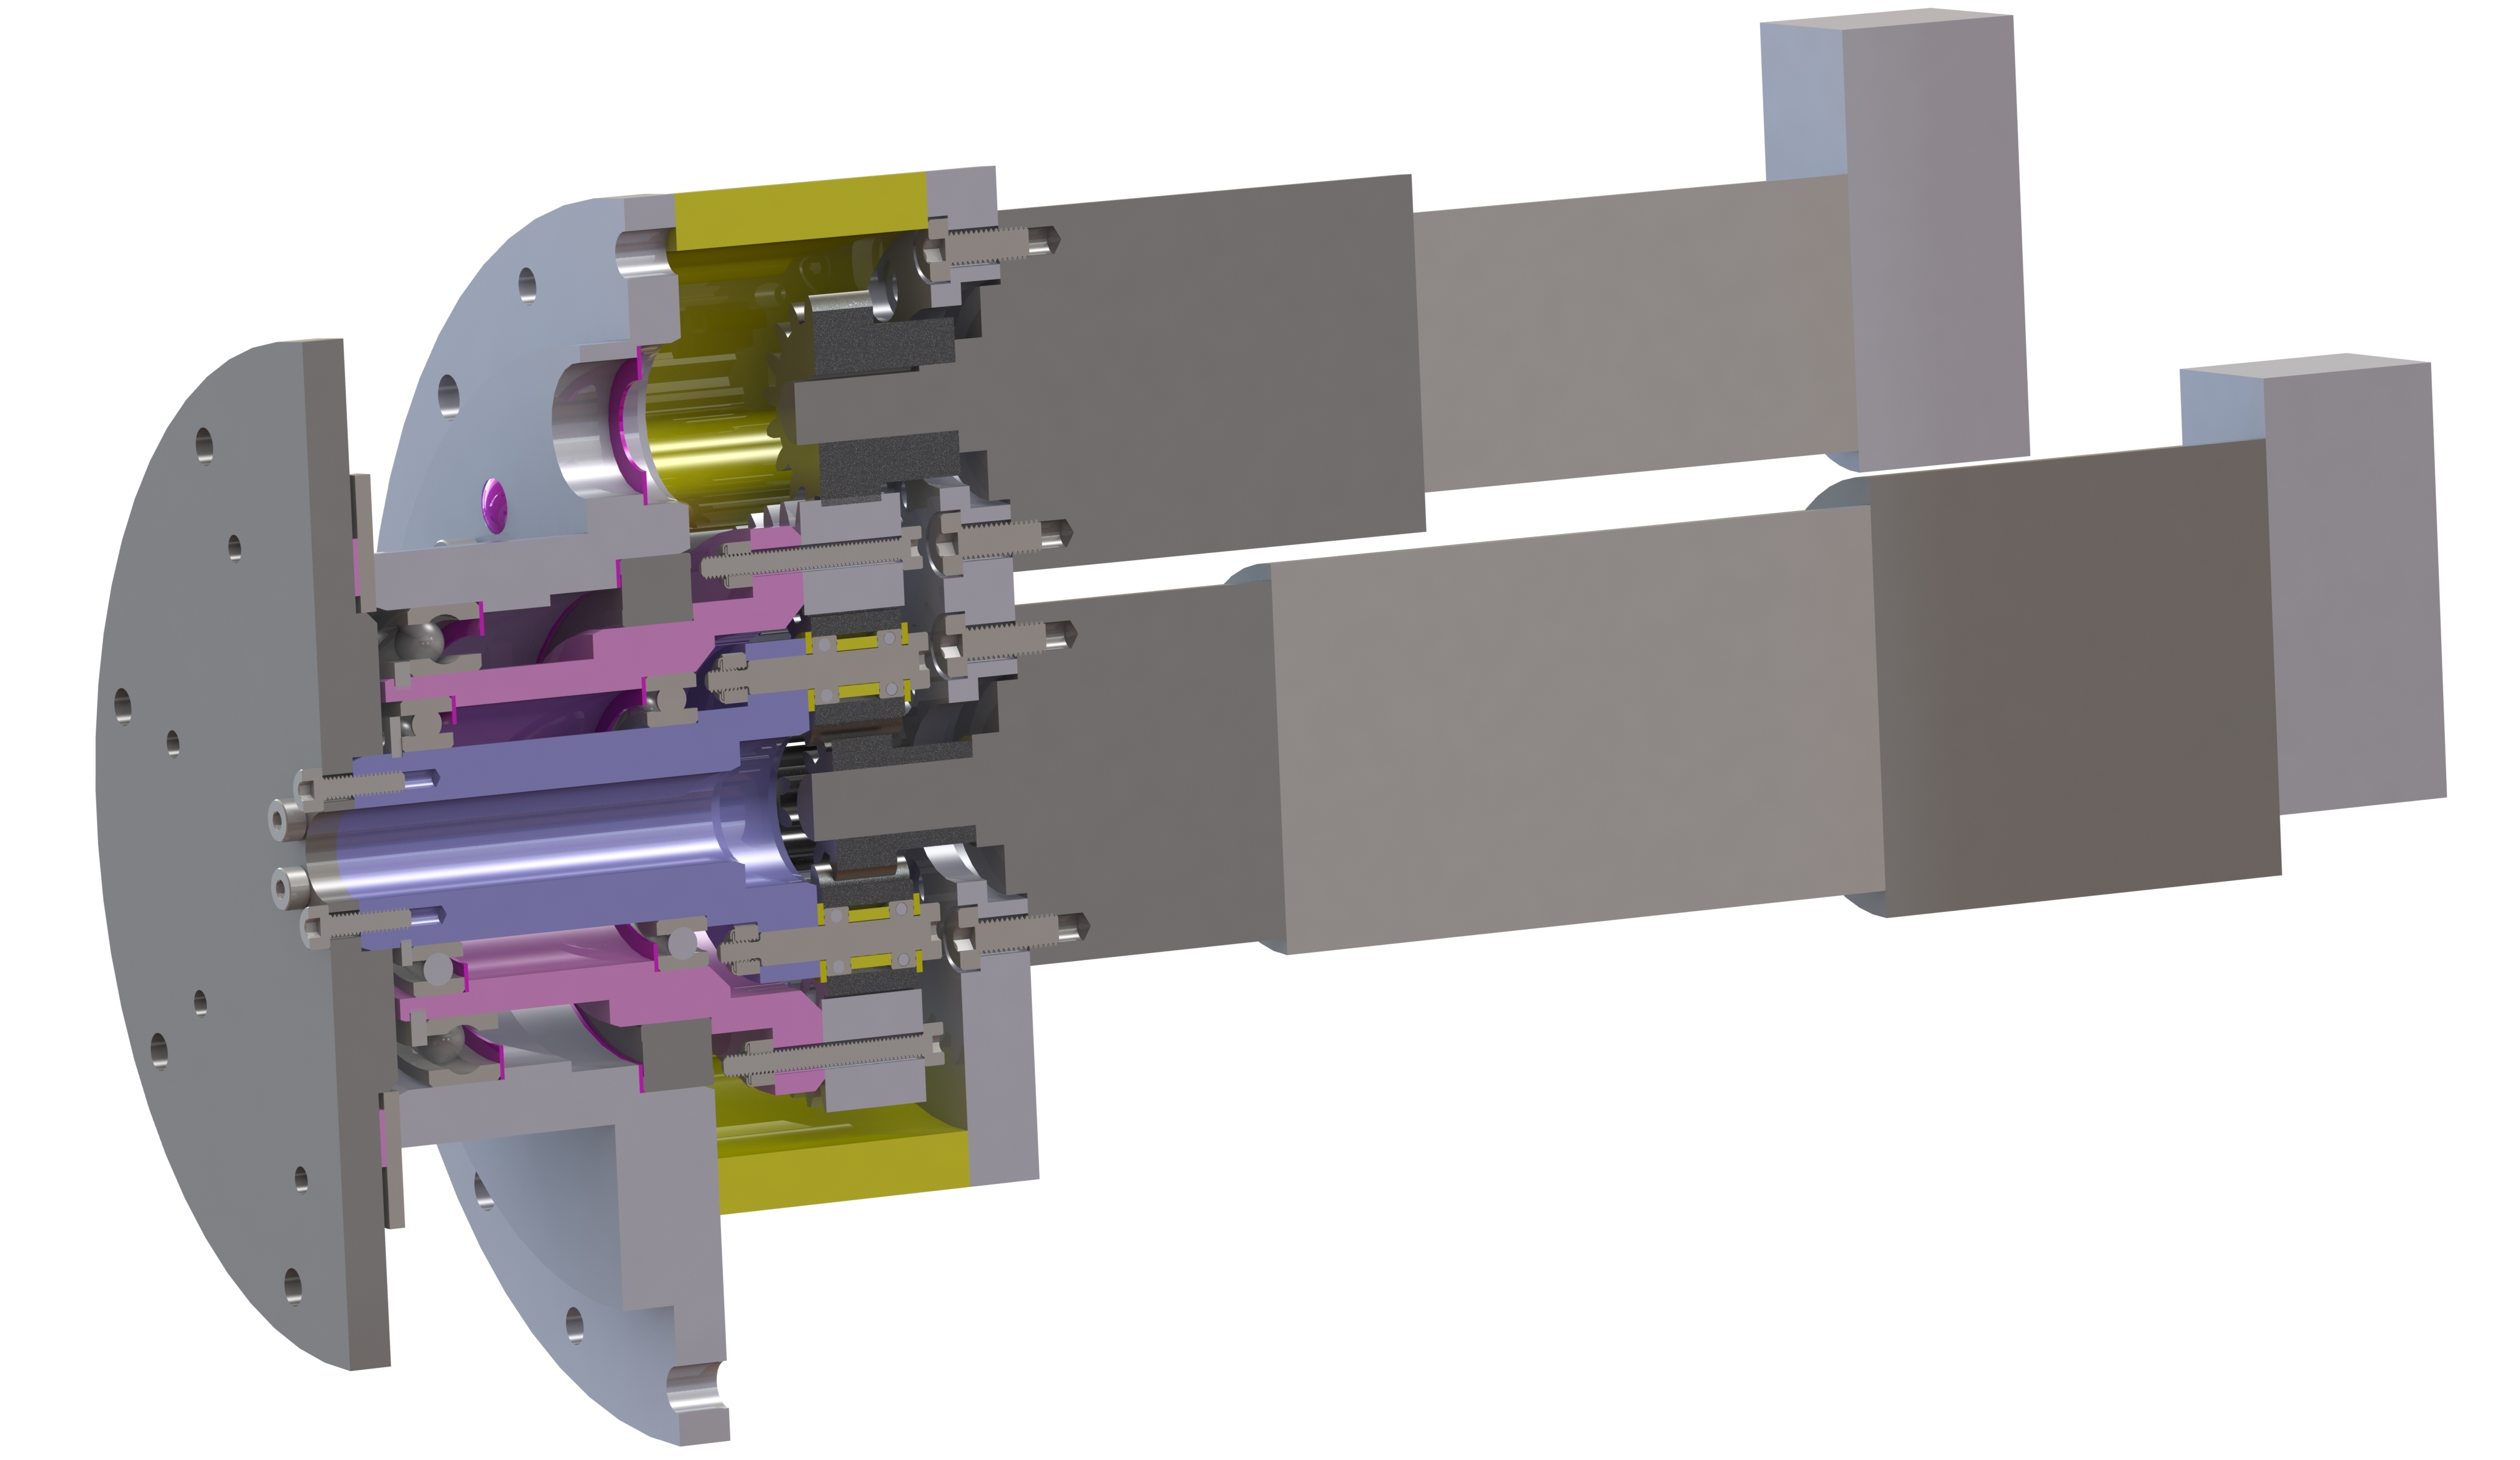
\includegraphics[width=0.95\textwidth]{metal_DSDM_section_view.jpg}
	\caption{Section view of the CAD model of the revolute actuator prototype} %Max continuous torque of 40 Nm and maximum velocity of 100 RPM
	\label{fig:dsdm_section}
\end{figure}

\begin{figure}[htbp]
	\centering
		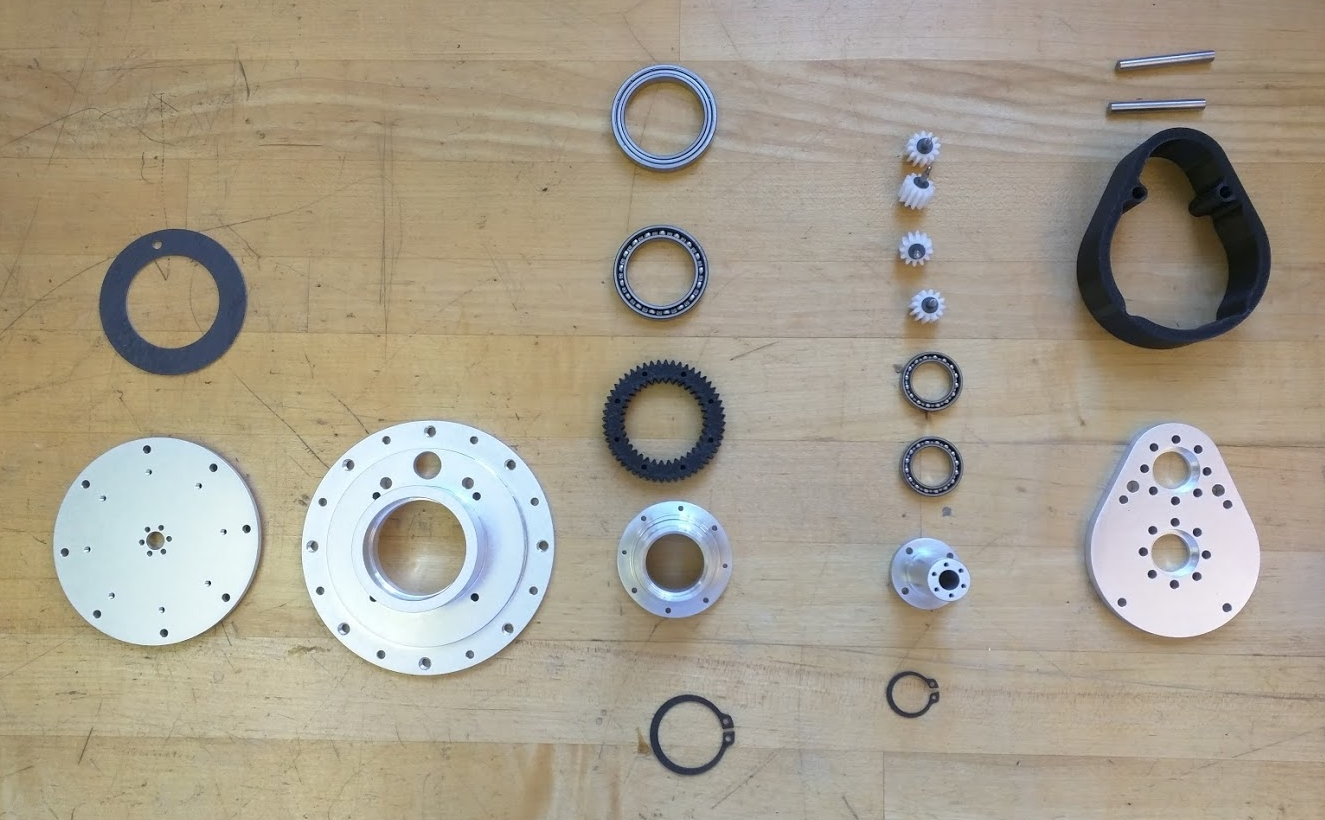
\includegraphics[width=0.90\textwidth]{dsdm_parts.jpg}
	\caption{Internal components of the revolute actuator prototype}
	\label{fig:dsdm_parts}
\end{figure}

A \textit{Maxon} motor of the series RE-25, with maximum continuous power of 20 watts and torque 0.03 Nm, is used for M2, and motor of the series RE-35, with maximum continuous power of 90 watts and torque 0.1 Nm, is used for M1. The revolute actuator prototypes use additional gear-head reduction for both motor, to increase both value of total reduction $R_1$ and $R_2$, to reach useful range of torque and speeds, as illustrated at Table \ref{tab:specrev}. 
%
\begin{table}[htbp]
	\centering
	\caption{Specifications of revolute actuator prototypes}
		\begin{tabular}{ c c c c c c c}
			\hline
			Role & $R_1$ & $R_2$ & M1 power & M2 power & Max. Torque & Max. Velocity \\
			\hline
			       & $\frac{w_1}{w_o}$ & $\frac{w_2}{w_o}$ & Watts & Watts & Nm & RPM \\
			\hline \hline
			Wrist & 23 & 474  & 100 & 20 & 14 & 220 \\
			Elbow & 72 & 1225 & 100 & 20 & 37 & 70 \\
			\hline
		\end{tabular}
	\label{tab:specrev}
\end{table}
 
Note that the ratio $R_2/R_1$ is always keep at a factor of about 20, to match the capability of the brake according to eq. \eqref{eq:brakelim}. Also, the specifications of maximum torque, are given in term of very conservative continuous value advertised by \textit{Maxon}. Better performance could be obtained in term of peak torque during short time periods. The whole assembly of embedded DSDM actuator and support bearings for the revolute joint weight about 1.5 Kg. About half of this weight is due to \textit{Maxon} motor assemblies (motors, gear-heads and brakes) and the other half is the custom built transmission and joint support. This value should not be taken as a state-of-art comparison reference to other actuation technologies since 1) no optimization for weight has been conducted, 2) industrial DC \textit{Maxon} motor are don't have the best available power density and 3) the design was focus on ease of implementation and modularity. 


\subsubsection{Linear Actuator}

To achieve the large reduction needed for the shoulder actuator of the robot, while keeping the mechanism back-drivable during high-speed mode, a large-lead ballscrew linear stage is used. Fig. \ref{fig:linact} shows the linear actuator assembly, and Fig. \ref{fig:dsdm_parts_old} shows the internal components. 

\begin{figure}[htp]
	\centering
		%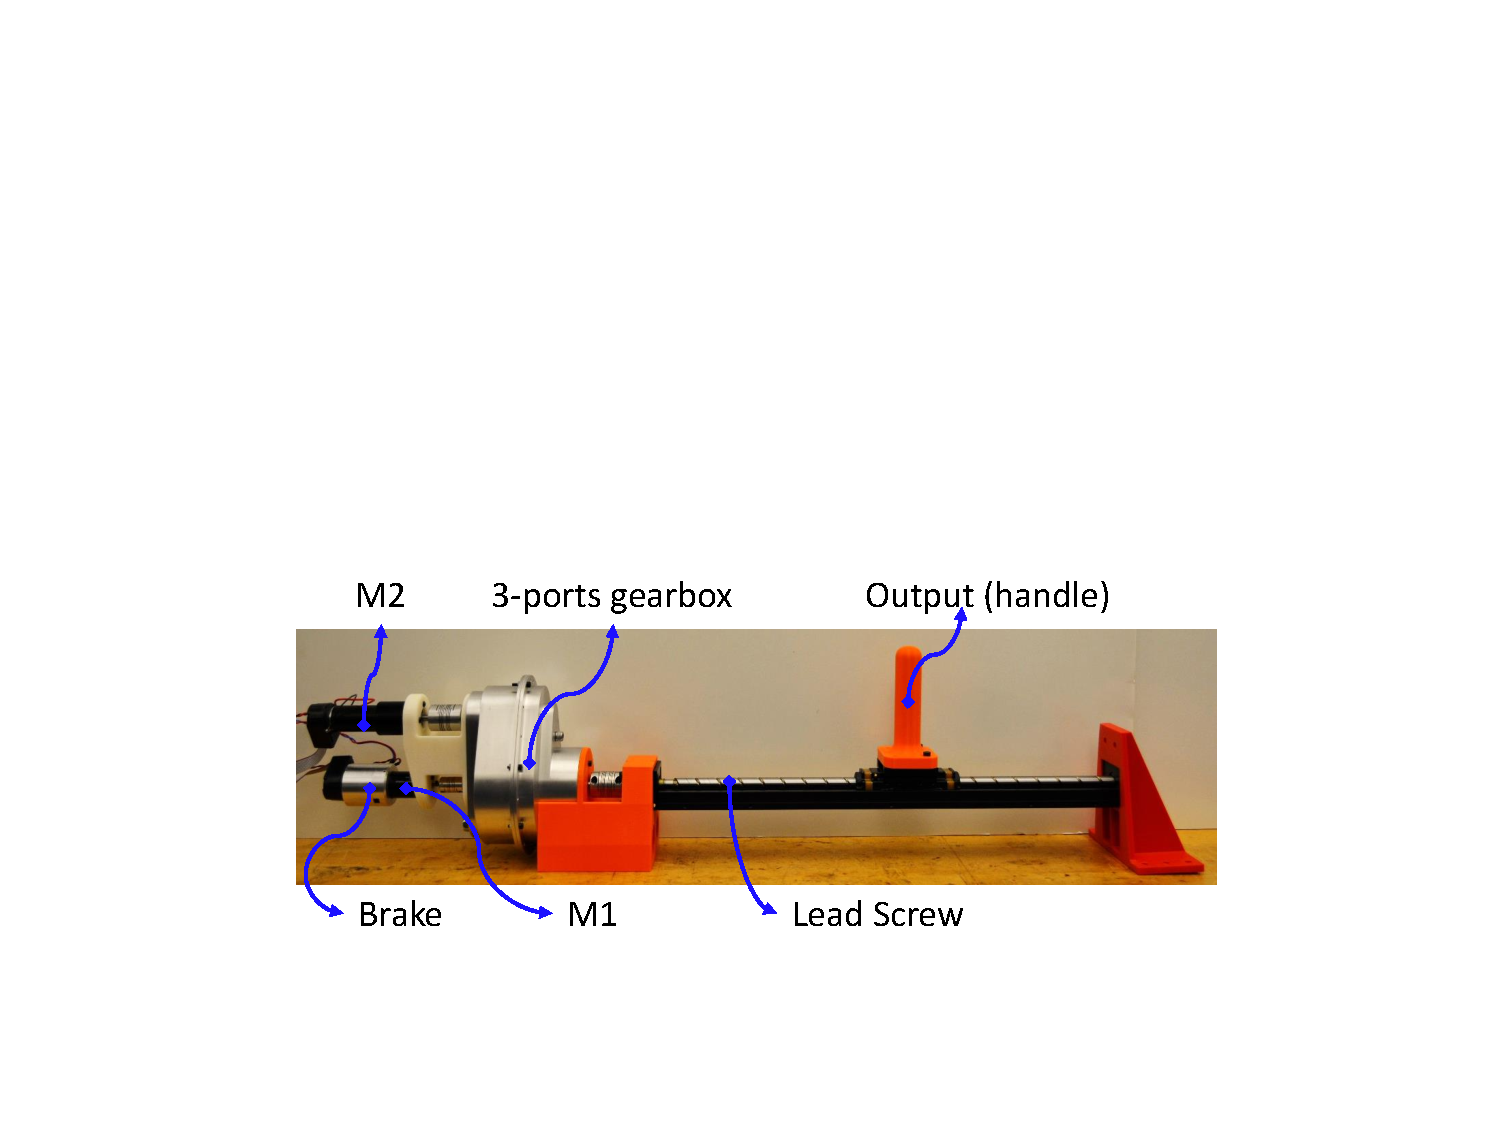
\includegraphics[width=0.95\textwidth]{proto_linear.pdf}
		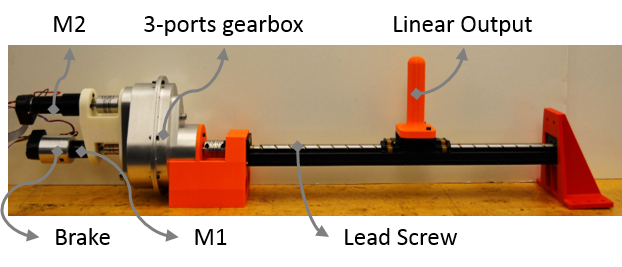
\includegraphics[width=0.95\textwidth]{DSDMpic.png}
	\caption{Linear actuator assembly in a preliminary test configuration} 
	\label{fig:linact}
\end{figure}

\begin{figure}[htbp]
	\centering
		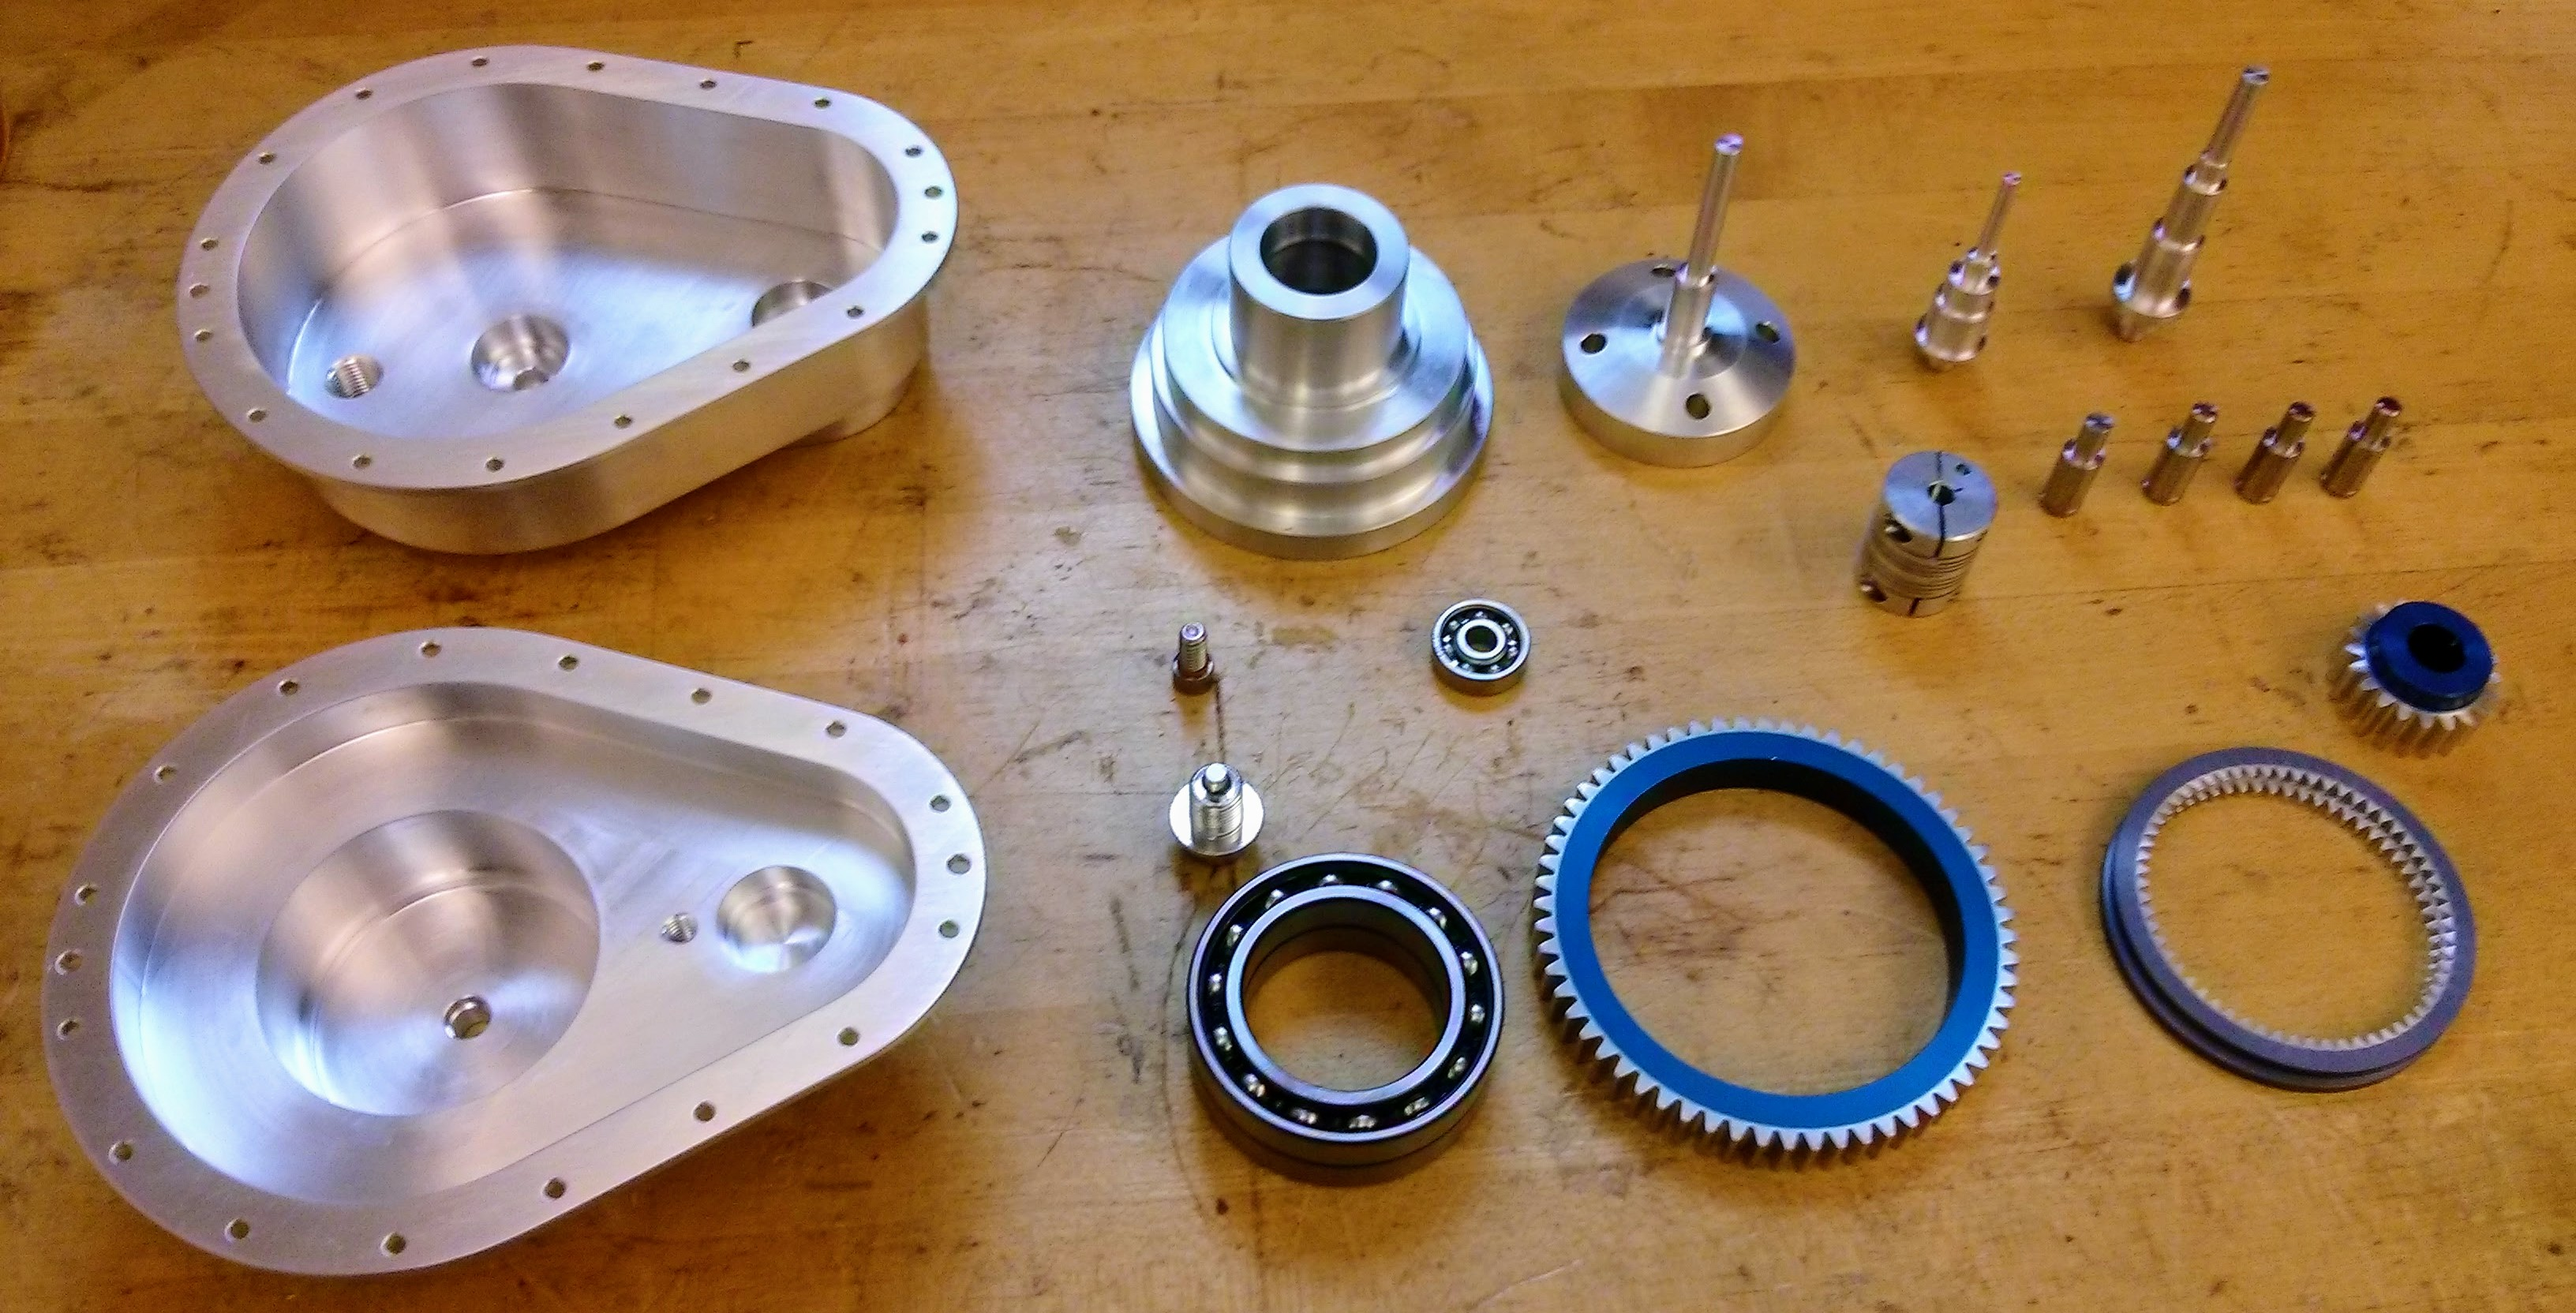
\includegraphics[width=0.90\textwidth]{dsdm_parts_old.jpg}
	\caption{Internal components of the DSDM linear actuator}
	\label{fig:dsdm_parts_old}
\end{figure}

The linear actuator assembly was initially designed as an experimental test bench for the DSDM technology \cite{girard_two-speed_2015}. Unlike the revolute actuators, the transmission is sealed and lubricated with oil and flexible coupling are used to connect all the components.  The linear actuator is thus more heavy duty, bigger and heavier than the revolute actuators. However, the linear actuator assembly is fixed to the ground and not a moving part of the DSDM-Arm, hence drawback of its weight and volume are limited. 

Two \textit{Maxon} RE-25 motors capable of continuous operation of 20 Watts and 0.03 Nm are used for both M1 and M2. Only M2 is equipped with a gear-head for the linear actuator; the reduction provided by the ball-screw and the differential are sufficient for the high-speed mode. Overall gear-ratios in the design and resulting specifications are given at Table. \ref{tab:speclin}.

\begin{table}[htbp]
	\centering
	\caption{Specifications of the linear actuator prototype}
		\begin{tabular}{ c c c c c c c }
			\hline
			$R_1$ & $R_2$ & Lead & M1 power & M2 power & Max. Force & Max. Velocity \\
			\hline
			$\frac{w_1}{w_o}$ & $\frac{w_2}{w_o}$ & mm/rev &Watts & Watts & N & m/s \\
			\hline \hline
			4 & 72 & 20 & 20 & 20 & 600 & 0.7 \\
			\hline
		\end{tabular}
	\label{tab:speclin}
\end{table}

It is interesting to note that any commercially available linear actuator matching similar specifications of force and speed are much bigger and heavier than the presented linear actuator prototype, even with this un-optimized design. With a single gear-ratio, commercial actuator would need to use a DC motor of roughly $0.7 \, \frac{m}{s} \times 600 N \; = \; 0.4 kW $, almost 2/3 of a horsepower. A \textit{Maxon} motor (in the same DC category) weight over 2 kg to meet those specifications, compared to two 20 W motor weighting each about 130g. Of course, the linear actuator with a single big motor would be much more powerful than the presented linear actuator, but such power might be unnecessary. There is a need for actuators that can be both fast and strong, not necessary powerful, and very lightweight. 


\subsection{Arm Design}
\label{sec:DSDMArm}

The DSDM-arm is built using very lightweight square tubing of carbon fiber. 3D printed plastic (ABS) parts are designed to make the junction between revolute joint assemblies and the tubes. The revolute joint assemblies are joined to printed parts with a bolt pattern, and printed parts are simply clamped on the square tubes. This allows for very quick reconfiguration of the arm, tubes of different lengths can be used and revolute joints can be mounted at different angles on the tubes. The carbon fiber tube between the shoulder and the elbow has a cross section of 2"x2" while the tubes linking elbow-wirst and wrist-end-effector have a 1"x1" cross section. 

\subsubsection{Shoulder 4-bar mechanism}

A 4-bar mechanism is designed to transmit the linear actuator motion to the revolute shoulder joint, see Fig. \ref{fig:4bar}. This combination of ballscrew with a 4-bar mechanism allows for a very large mechanical advantage to be achieved, and with very good transmission efficiency.  

\begin{figure}[htbp]
	\centering
		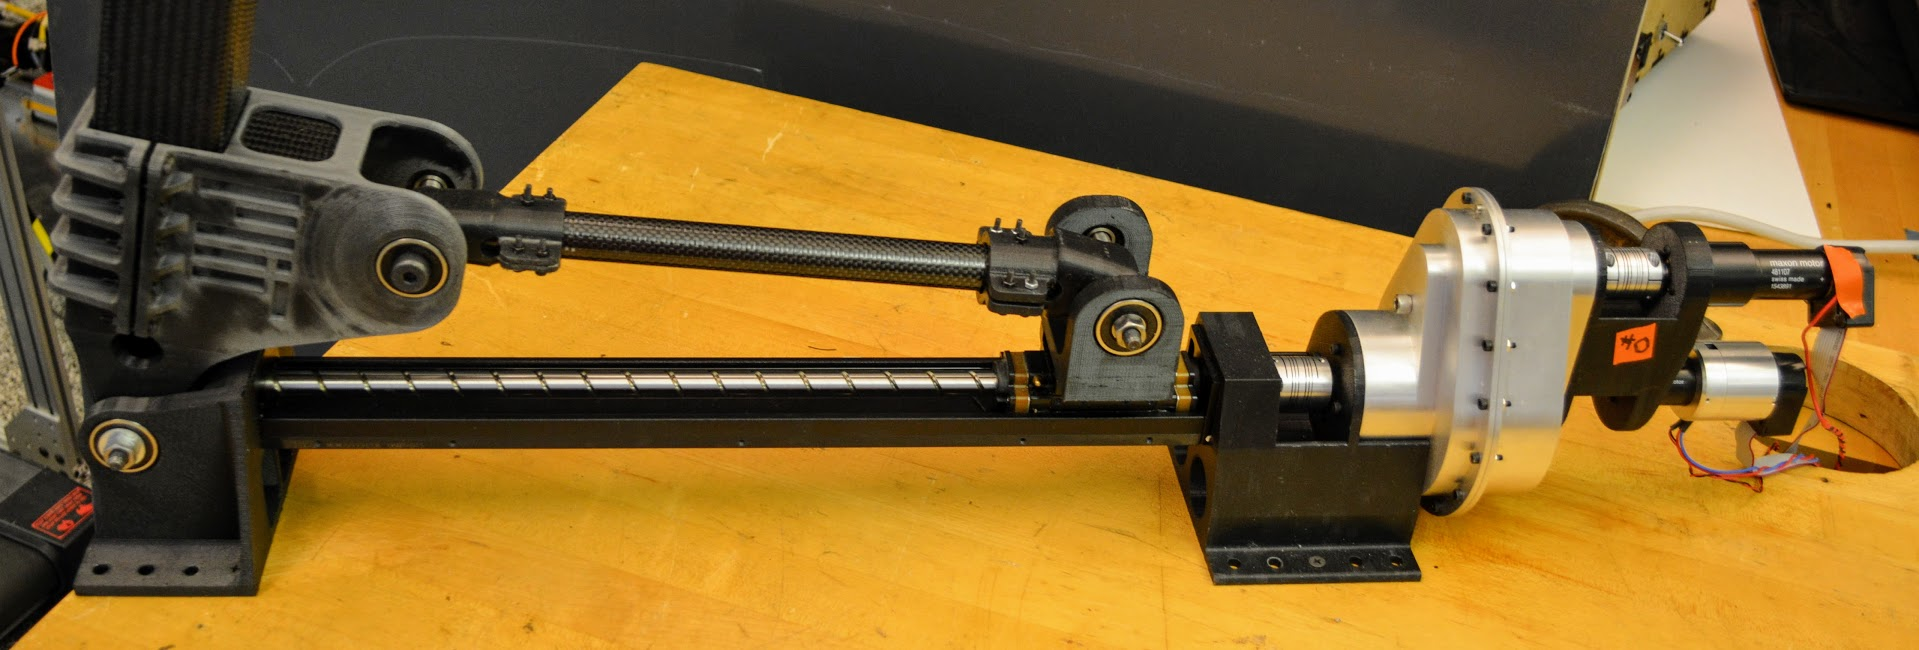
\includegraphics[width=0.95\textwidth]{4bar.jpg}
	\caption{Shoulder 4-bar mechanism}
	\label{fig:4bar}
\end{figure}

The geometry of the 4-bar mechanism has been designed to achieve the desired range of angles for the shoulder, and keeping the kinematic relationship, between linear displacement and shoulder angle, as linear as possible. Fig. \ref{fig:shoulder_kinematic} illustrates the kinematic relationship of the designed mechanism. Note that in the software controlling the arm, this kinematic relationship is computed explicitly for the inverse-kinematic but the forward kinematic is approximated with a numerical interpolation (when computing the shoulder position based on encoder measurements of the linear actuator). The shoulder forward kinematic has a unique solution for the range of physically possible linear actuator displacement.

\begin{figure}[htbp]
	\centering
		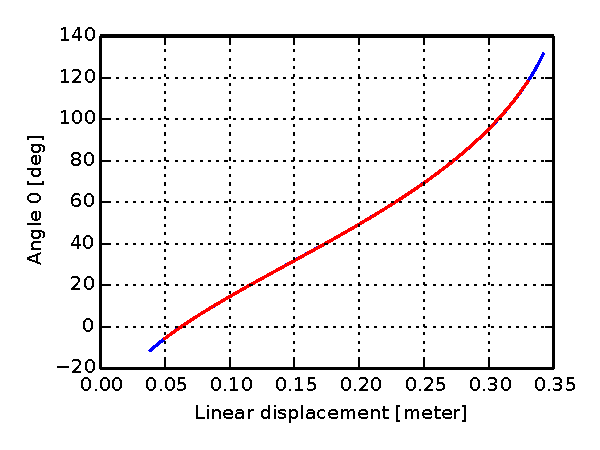
\includegraphics[width=0.65\textwidth]{shoulder_kinematic.pdf}
	\caption{Shoulder 4-bar mechanism kinematic}
	\label{fig:shoulder_kinematic}
\end{figure}

The mechanical advantage between linear motion and shoulder rotation is thus on average about 360 deg/m, or a ratio of 50:1 from ballscrew rotation to shoulder rotation. This correspond to average total reduction ratios of $R_1 = 200 $ and $R_2 = 3600 $. Surprisingly, the shoulder joint mechanism is backdrivable, even during high-force mode. This illustrates the efficiency of ballscrew-based reduction mechanisms. During high-speed mode, a human can easily move the first joint of the robot with almost no resistance. During high-force mode, the reflected inertia is very large, but a human can still make the shoulder joint move very slowly by pushing hard (with open circuit for the motor). However, if there is a small damping force at M2 motor shaft (by closing the motor electric circuit for instance), than back-driving the system is almost impossible.  


\subsubsection{Arm Specifications} 

Table \ref{tab:robotspec} shows the arm specifications at the joints in term of force, speed and reflected motor inertia. Table \ref{tab:robotspec2}, shows the DSDM arm joint specifications transposed to end-effector space where they are more meaningful. For doing so, a configuration where all link are aligned and tube lengths of 0.5 m, 0.25 m and 0.25 m is assumed, see Fig. \ref{fig:arm_config}. Then the maximum force, maximum speed and impedance at the end-point, due to each actuator taken independently, are computed. All in all, with the designed reduction ratios, during high-speed mode the end-point inertia due to reflected motors inertia is negligible and speed can reach multiple meters per second. With the high-force mode, the end-point force capability reach 50 N (limited by the wrist) even in this most disadvantageous fully extended configuration, with the end-effector at arms' length.  

\begin{table}[htbp]
	\centering
	\caption{DSDM-Arm Joint Specifications}
		\begin{tabular}{ c c c c c c c c c c }
			\hline
			   & Range  & \multicolumn{2}{c}{Reduction} & \multicolumn{2}{c}{Max. Velocity} & \multicolumn{2}{c}{Max. Torque} & \multicolumn{2}{c}{Inertia} \\
			   & deg & & &\multicolumn{2}{c}{RPM} & \multicolumn{2}{c}{Nm} & \multicolumn{2}{c}{kg m$^2$} \\
				\hline 
			  & & HF & HS & HF & HS & HF & HS & HF & HS \\
			\hline
			 Wrist & $\infty$ & 474:1  & 23:1  & 10 & 220 & 14  & 2 & 0.22 & 0.004 \\
			 Elbow & $\infty$ & 1225:1 & 72:1  & 4  & 70  & 37  & 7 & 1.5  & 0.04  \\
			 Shoulder & 120   & 3600:1 & 200:1 & 1  & 25  & 108 & 6 & 13   & 0.04  \\
			\hline
		\end{tabular}
	\label{tab:robotspec}
\end{table}

\begin{figure}[htb]
	\centering
		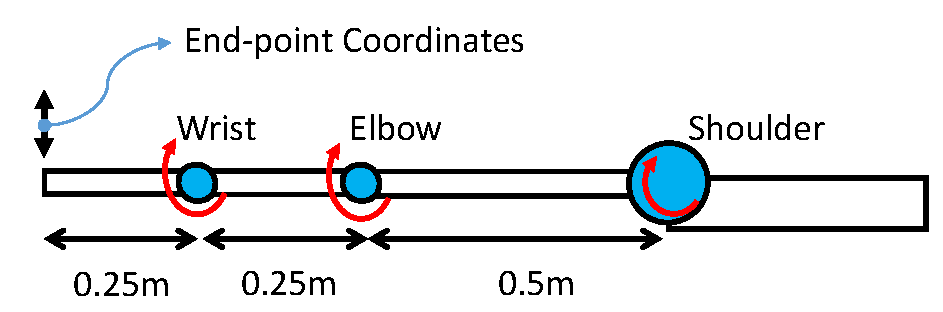
\includegraphics[width=0.65\textwidth]{arm_config.pdf}
	\caption{Arm configuration used to compute end-point specifications}
	\label{fig:arm_config}
\end{figure}

\begin{table}[htpb]
	\centering
	\caption[DSDM-Arm End-point Specifications]{DSDM-Arm End-point Specifications with Configuration of Fig. \ref{fig:arm_config}}
		\begin{tabular}{ c c c c c c c }
			\hline
			   & \multicolumn{2}{c}{Max. Velocity} & \multicolumn{2}{c}{Max. Force} & \multicolumn{2}{c}{Reflected Mass}\\
			   & \multicolumn{2}{c}{m/s} & \multicolumn{2}{c}{N} & \multicolumn{2}{c}{kg } \\
				\hline
			  & HF & HS & HF & HS & HF & HS \\
			\hline
			 Wrist    & 0.25 & 5    & 56  &  8  & 3.5 & 0.06   \\
			 Elbow    & 0.2  & 3.5  & 74  &  14 & 6   & 0.16    \\
			 Shoulder & 0.1  & 2.5  & 108 &  6  & 13  & 0.04    \\
			\hline
		\end{tabular}
	\label{tab:robotspec2}
\end{table}

Note that the DSDM-Arm is strong enough to sustain its own weight in all configurations when using high-force (HF) modes. However, this is not the case when using the actuators in high-speed (HS) mode. 


\subsection{Limitations and recommendations for improvements} 

The main limitations of the DSDM-Arm are due to 1) backlash in the actuator gearing and 2) compliance in the structure. For the ease of implementation, the custom built actuator transmissions use only standard spur gears. The flaw of this design is that the output has a backlash of a few degrees. While it was not a critical issue for demonstrating the proposed control scheme of this thesis, it would be problematic for using the DSDM-Arm platform in task involving precise positioning of the end-effector. The second issue is the arm compliance due to 3D printed plastic parts used to connect the joints to the carbon fiber tubes. 

Regarding the backlash in the gearing, this could be avoided by spending more engineering effort to make thorough precision gear-box design. For the compliance in the structure, using metal parts could solve the issue but would lead to a heavier robotic system. Instead, it would be interesting to use 3D printed parts reinforced with carbon fiber, such as the \textit{Markforged} technology. 



%%%%%%%%%%%%%%%%%%%%%%%%%%%%%%%%%%%%%%%%%%%%%%%%%%%%%%%%%%%%%%%%%%%%%%%%%%%%%%%%%%%%%%%

\newpage
\newpage

\section{Control and Software Architecture}
\label{sec:ControlSoftwareArchitecture}

This section discusses implementation of the control algorithms for the DSDM-Arm. 

\subsection{Global Architecture}

Fig. \ref{fig:archi_diagram} illustrates the hierarchical control architecture for the DSDM-Arm. At the very high-level an operator gives commands to the system using a wireless \textit{xbox-360} controller, and at the very low level, pwm signal are sent to motor power-electronic circuits. The physical platforms include a desktop computer running Ubuntu 14.04 and ROS \cite{quigley_ros:_2009}, and multiple micro-controllers. 

\begin{figure}[H]
	\centering
		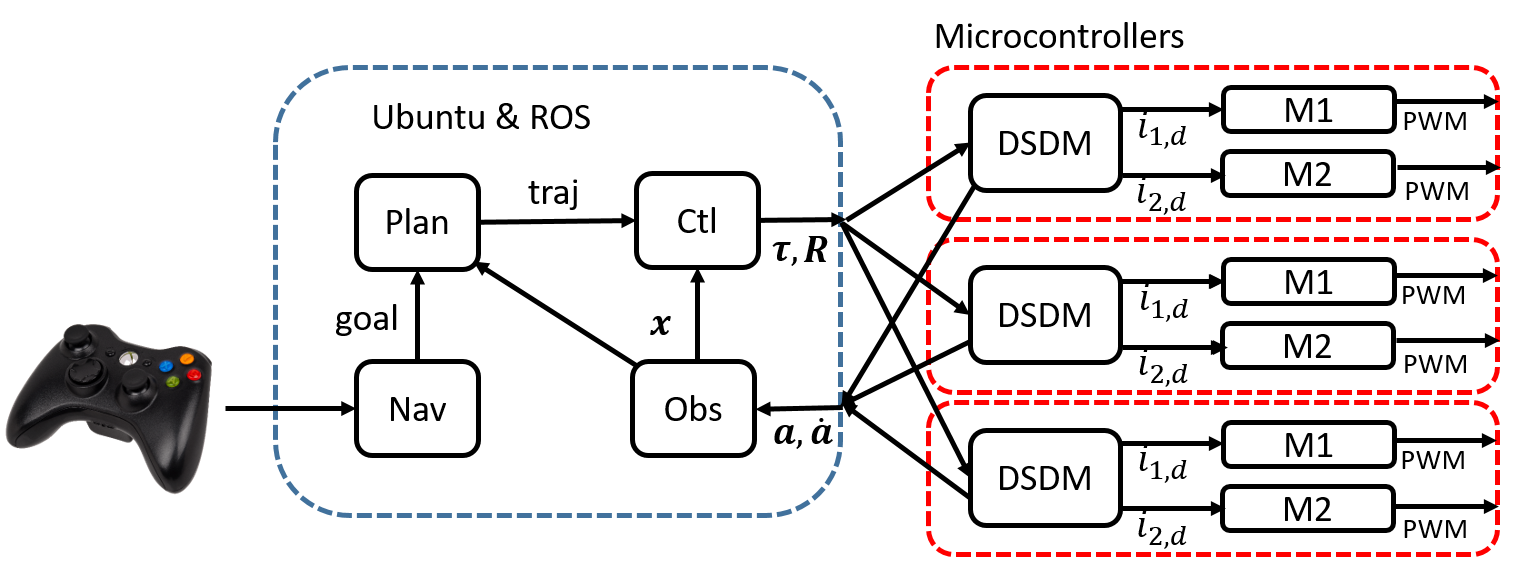
\includegraphics[width=0.95\textwidth]{ros_diagram.png}
	\caption{Control Software Architecture}
	\label{fig:archi_diagram}
\end{figure}

The high-level motion planning algorithm, the centralized robot controller is running on the desktop. Each motor as its own micro-controller handling the low-level current control loop. The plan for the DSDM controllers, was to decentralize them on one individual micro-controllers for each actuators. However, at the time of writing these lines, all three DSDM controllers are programs running on the desktop, which communicates directly with the six motor boards. Communication between the desktop and motor micro-controllers is done over USB connections.

\subsection{ROS Architecture}

Fig. \ref{fig:ros_3dsdm} and \ref{fig:ros_dsdm} illustrates the software architecture in ROS, those figures were generated directly from ROS using the \textit{rqt\_graph} command. Each ellipse, nodes using the ROS nomenclature, represent an independent program, and arrows represent communication pipelines in between those programs, topics using the ROS nomenclature. All programs were written in \textit{python} with the exception of the FlexSEA drivers, handling the communication with motor micro-controllers, which are written in \textit{C++}.

\begin{figure}[htpb]
	\centering
		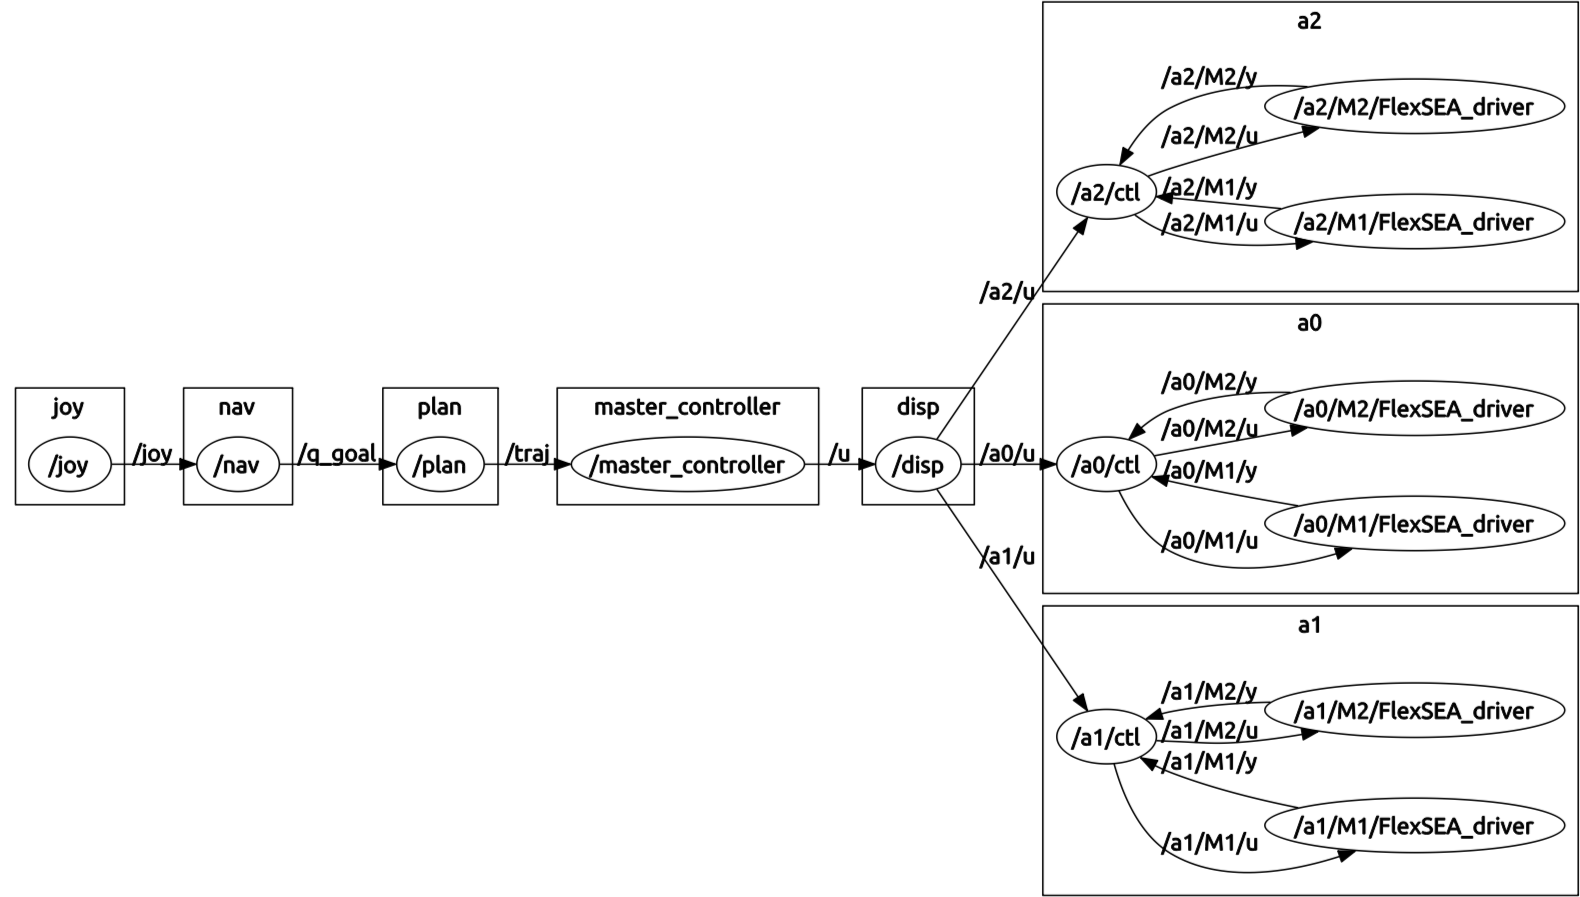
\includegraphics[width=0.95\textwidth]{ros_graph_3_dsdm.png}
	\caption{ROS architecture for the full robot (feedback connections are omitted)}
	\label{fig:ros_3dsdm}
\end{figure}

\begin{figure}[htpb]
	\centering
		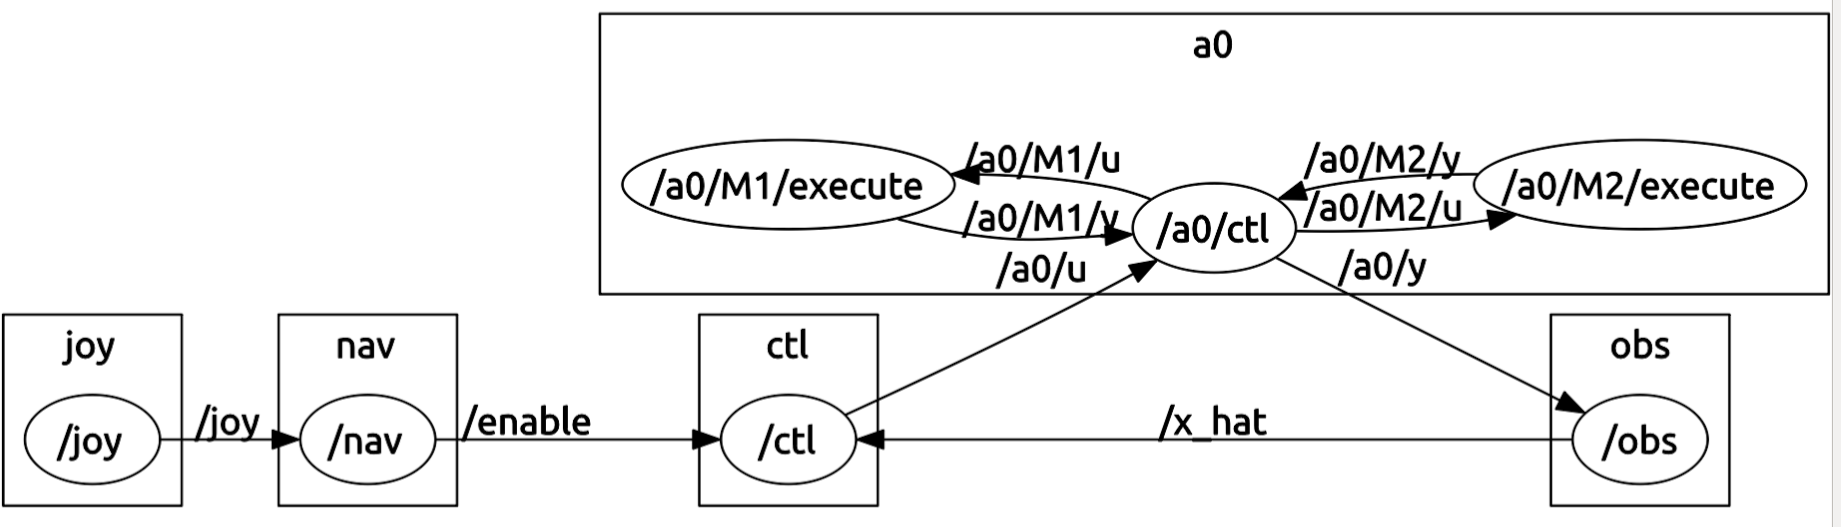
\includegraphics[width=0.85\textwidth]{ros_graph_single_dsdm.png}
	\caption{ROS architecture for controlling a single DSDM actuator directly}
	\label{fig:ros_dsdm}
\end{figure}


\subsection{Navigation}

The \textit{joy} node read button states of the wireless controller, and broadcast them when button state changes. This program is available as an open-source ROS package. The \textit{nav} node then maps buttons to operating modes and desired goals. Multiple operating modes are available: sending a configuration goal to the planner, sending a reference directly to the robot controller, or manually controlling actuator torques and gear-ratios. 

\subsection{Trajectory Planning}

The \textit{plan} node implement the RRT algorithm, as described in sec. \ref{sec:SamplingBasedTrajectoryPlanner}, to generate feasible trajectories. When receiving a new configuration goal, the node reads the current states, search for a feasible trajectory, and then broadcast the reference trajectory solution. Execution time of the search is stochastic, but is on the order of about 1 sec for 1-DoF systems and 10 sec for 2-DoF systems, with the custom implementation.

\subsection{State feedback}

The FlexSEA driver nodes are programed to continuously request and receive encoder measurements from motor boards at a rate of 500 Hz. The DSDM controller nodes then read those values, process them (kinematic relationship based on gear-ratios and filtered differentiation to compute velocities), and broadcast position and velocity of actuator output coordinates. The \textit{obs} node then read all actuator measurements and transposes them to joint coordinates. This step is trivial except for the 4-bar mechanism of the shoulder joint for which an interpolation function synthesized offline is used. 

\subsection{Robot Controller}

The master robot controller, loads a reference trajectory, and compute actuator torques and gear-ratios in closed-loop based on state feedback at the rate of 500 Hz. Multiple control policies from chapter \ref{sec:ControlAndPlanningOfRobotUsingVariableGearRatioActuators} are implemented:
%
\begin{itemize}
	\item R* Computed Torque controller
	\item R* Sliding Mode Controller
	\item Rollout gear-selection
\end{itemize}
%
For controlling only 1-DoF with two gear-ratios options, the Rollout gear-selection can run with a time horizon of 1-2 sec without slowing down the 500 Hz rate of the controller. However, when running the controller for 2-DoF with four gear-ratios options, the predictive simulations had to be simplified by using very rough integration steps for the scheme to run at 500 Hz. This should not be taken as a computational limit of the approach since here non-optimized inefficient \textit{python} code was used.

\subsection{DSDM Actuator Controllers}

DSDM controllers are currently implemented as ROS nodes. They receive a torque and a gear-ratio command from the master robot controller and send current set-points and brake command to the motor drivers, also at 500 Hz. DSDM controller nodes implement the control schemes described in Chapter \ref{sec:MultipleSpeedActuationTechnology}.

\subsection{Motor drivers}

The motor are controlled by open-source FlexSEA Execute motor board \cite{duval_flexsea-execute:_2016}. Those boards handle low-level high-bandwidth current loops and encoder signal processing. They also include a circuit to control a brake. All those functions are made available from the FlexSEA driver nodes. Here the driver are set to request, receive and broadcast all sensor information from the Execute boards constantly at 500 Hz, which set the tempo for the feedback loops. 


\subsection{Limitations and recommendations for improvements} 

The initial control implementation for DSDM actuator prototypes used a \textit{NI compact rio} where feedback loops were running at very high-sampling rate on a FPGA and a real-time micro-controller \cite{girard_two-speed_2015}. This type of system was however poorly suited to scale to multi-DoF systems, and implementing complex planning algorithms. Hence, for the DSDM-Arm the architecture was design to: easily scale to multiple DoF, make possible the use of high-level programming languages and facilitate connections with motion planning algorithms. However this came at the cost of losing some control on the low-level control loops implementations. The performance of actuator-level DSDM controller has decreased with the new implementation. To improve the system, DSDM controllers should be implemented directly on micro-controllers, handling all actuator-level functions, at a higher sampling rate. One implementation issue that could also be improved, is that velocity measurements, at low speeds in high-speed mode, are very noisy because of resolution problems. An encoder with improved resolution, or direct an angular velocity sensor should be used to improve the performance. 








